\newcommand{\byr}{Br}

\section{Технико-экономическое обоснование эффективности разработки мобильного программного средства <<Органайзер здоровья пациента>>}

% Begin Calculations

\FPeval{\totalProgramSize}{15680}
\FPeval{\totalProgramSizeCorrected}{8650}

\FPeval{\normativeManDays}{224}

\FPeval{\additionalComplexity}{0.12}
\FPeval{\complexityFactor}{clip(1 + \additionalComplexity)}

\FPeval{\stdModuleUsageFactor}{0.7}
\FPeval{\originalityFactor}{0.7}

\FPeval{\adjustedManDaysExact}{clip( \normativeManDays * \complexityFactor * \stdModuleUsageFactor * \originalityFactor )}
\FPround{\adjustedManDays}{\adjustedManDaysExact}{0}

\FPeval{\daysInYear}{365}
\FPeval{\redLettersDaysInYear}{9}
\FPeval{\weekendDaysInYear}{104}
\FPeval{\vocationDaysInYear}{21}
\FPeval{\workingDaysInYear}{ clip( \daysInYear - \redLettersDaysInYear - \weekendDaysInYear - \vocationDaysInYear ) }

\FPeval{\developmentTimeMonths}{3}
\FPeval{\developmentTimeYearsExact}{clip(\developmentTimeMonths / 12)}
\FPround{\developmentTimeYears}{\developmentTimeYearsExact}{2}
\FPeval{\requiredNumberOfProgrammersExact}{ clip( \adjustedManDays / (\developmentTimeYears * \workingDaysInYear) + 0.5 ) }

% тут должно получаться 2 ))
\FPtrunc{\requiredNumberOfProgrammers}{\requiredNumberOfProgrammersExact}{0}

\FPeval{\tariffRateFirst}{600000}
\FPeval{\tariffFactorFst}{3.04}
\FPeval{\tariffFactorSnd}{3.48}


\FPeval{\employmentFstExact}{clip( \adjustedManDays / \requiredNumberOfProgrammers )}
\FPtrunc{\employmentFst}{\employmentFstExact}{0}

\FPeval{\employmentSnd}{clip(\adjustedManDays - \employmentFst)}


\FPeval{\workingHoursInMonth}{160}
\FPeval{\salaryPerHourFstExact}{clip( \tariffRateFirst * \tariffFactorFst / \workingHoursInMonth )}
\FPeval{\salaryPerHourSndExact}{clip( \tariffRateFirst * \tariffFactorSnd / \workingHoursInMonth )}
\FPround{\salaryPerHourFst}{\salaryPerHourFstExact}{0}
\FPround{\salaryPerHourSnd}{\salaryPerHourSndExact}{0}

\FPeval{\bonusRate}{1.5}
\FPeval{\workingHoursInDay}{8}
\FPeval{\totalSalaryExact}{clip( \workingHoursInDay * \bonusRate * ( \salaryPerHourFst * \employmentFst + \salaryPerHourSnd * \employmentSnd ) )}
\FPround{\totalSalary}{\totalSalaryExact}{0}

\FPeval{\additionalSalaryNormative}{20}

\FPeval{\additionalSalaryExact}{clip( \totalSalary * \additionalSalaryNormative / 100 )}
\FPround{\additionalSalary}{\additionalSalaryExact}{0}

\FPeval{\socialNeedsNormative}{0.5}
\FPeval{\socialProtectionNormative}{34}
\FPeval{\socialProtectionFund}{ clip(\socialNeedsNormative + \socialProtectionNormative) }

\FPeval{\socialProtectionCostExact}{clip( (\totalSalary + \additionalSalary) * \socialProtectionFund / 100 )}
\FPround{\socialProtectionCost}{\socialProtectionCostExact}{0}

\FPeval{\taxWorkProtNormative}{4}
\FPeval{\taxWorkProtCostExact}{clip( (\totalSalary + \additionalSalary) * \taxWorkProtNormative / 100 )}
\FPround{\taxWorkProtCost}{\taxWorkProtCostExact}{0}
\FPeval{\taxWorkProtCost}{0} % это считать не нужно, зануляем чтобы не менять формулы

\FPeval{\stuffNormative}{3}
\FPeval{\stuffCostExact}{clip( \totalSalary * \stuffNormative / 100 )}
\FPeval{\stuffCost}{\stuffCostExact}

\FPeval{\timeToDebugCodeNormative}{15}
\FPeval{\reducingTimeToDebugFactor}{0.3}
\FPeval{\adjustedTimeToDebugCodeNormative}{ clip( \timeToDebugCodeNormative * \reducingTimeToDebugFactor ) }

\FPeval{\oneHourMachineTimeCost}{5000}

\FPeval{\machineTimeCostExact}{ clip( \oneHourMachineTimeCost * \totalProgramSizeCorrected / 100 * \adjustedTimeToDebugCodeNormative ) }
\FPround{\machineTimeCost}{\machineTimeCostExact}{0}

\FPeval{\businessTripNormative}{15}
\FPeval{\businessTripCostExact}{ clip( \totalSalary * \businessTripNormative / 100 ) }
\FPround{\businessTripCost}{\businessTripCostExact}{0}

\FPeval{\otherCostNormative}{20}
\FPeval{\otherCostExact}{clip( \totalSalary * \otherCostNormative / 100 )}
\FPround{\otherCost}{\otherCostExact}{0}

\FPeval{\overheadCostNormative}{100}
\FPeval{\overallCostExact}{clip( \totalSalary * \overheadCostNormative / 100 )}
\FPround{\overheadCost}{\overallCostExact}{0}

\FPeval{\overallCost}{clip( \totalSalary + \additionalSalary + \socialProtectionCost + \taxWorkProtCost + \stuffCost + \machineTimeCost + \businessTripCost + \otherCost + \overheadCost ) }

\FPeval{\supportNormative}{30}
\FPeval{\softwareSupportCostExact}{clip( \overallCost * \supportNormative / 100 )}
\FPround{\softwareSupportCost}{\softwareSupportCostExact}{0}


\FPeval{\baseCost}{ clip( \overallCost + \softwareSupportCost ) }

\FPeval{\profitability}{35}
\FPeval{\incomeExact}{clip( \baseCost / 100 * \profitability )}
\FPround{\income}{\incomeExact}{0}

\FPeval{\estimatedPrice}{clip( \income + \baseCost )}

\FPeval{\localRepubTaxNormative}{3.9}
\FPeval{\localRepubTaxExact}{clip( \estimatedPrice * \localRepubTaxNormative / (100 - \localRepubTaxNormative) )}
\FPround{\localRepubTax}{\localRepubTaxExact}{0}
\FPeval{\localRepubTax}{0}

\FPeval{\ndsNormative}{20}
\FPeval{\ndsExact}{clip( (\estimatedPrice + \localRepubTax) / 100 * \ndsNormative )}
\FPround{\nds}{\ndsExact}{0}


\FPeval{\sellingPrice}{clip( \estimatedPrice + \localRepubTax + \nds )}

\FPeval{\taxForIncome}{18}
\FPeval{\incomeWithTaxes}{clip(\income * (1 - \taxForIncome / 100))}
\FPround\incomeWithTaxes{\incomeWithTaxes}{0}

% End Calculations

\subsection{Характеристика программного продукта }

Предлагаемый для внедрения программный продукт является автоматизированной мобильной информационной системой ведения карточек пациента. Данная система осуществляет учет и регистрацию различного рода заболевания пациента на территории Республики Беларусь по средствам мобильного телефона. Эта разработка оказывает огромное  влияние на область медицины, ведь это позволяет автоматизировано вести картотеку пациента, тем самым позволяя во-время реагировать на определенные отклонения здоровья пациента.

Разработка продукта осуществлена в IT-компании «Иссофт Солюшенз» по индивидуальному заказу. В результате внедрения предлагаемой системы удается достичь:

\begin{itemize}
  \item повышения эффективности работы медицинских сотрудников и медицинских учреждений в целом;
  \item предоставление в доступном виде информацию полной картотеки пользователю-пациенту;
  \item сокращения нецелевых расходов интеллектуальной деятельности;
  \item предоставления качественного и количественного хранения информационного обеспечения;
\end{itemize}

Разработка данного проекта связана со значительными затратами трудовых и финансовых ресурсов. В связи с этим создание и реализация данного проекта нуждается в соответствующем технико-экономическом обосновании.

Целью технико-экономического обоснования является расчет и оценка следующих показателей:

\begin{itemize}
  \item смета затрат и отпускная цена ПО;
  \item прибыль от реализации ПО;
  \item рентабельность инвестиций в разработку ПО;
\end{itemize}

В результате разработки данного программного продукта снизится трудоемкость заполнения бумажной картотеки заболеваний пациента, что и будет являться результатом от внедрения программного продукта.

\subsection{Определение объема и трудоемкости ПО }

\subsubsection{Объем ПО. }

Базой для расчета плановой сметы затрат на разработку ПО является объем ПО.   

\subsubsection{Общий объем ($ V_{o} $)  }
программного продукта определяется исходя из количества и объема функций, реализуемых программой:

\begin{equation}
  \label{eq:econ:total_program_size}
  V_{o} = \sum_{i = 1}^{n} V_{i} \text{\,,}
\end{equation}
\begin{explanation}
где & $ V_{i} $ & объём отдельной функции ПО, LoC; \\
    & $ n $ & общее число функций.
\end{explanation}

\subsubsection{Единицы измерения объема ПО. }
Оценивание объема программного
продукта связано с выбором наиболее подходящей единицы измерения размера продукта. В данном обосновании будет использоваться количество строк исходного кода (LinеsОfСоdе, LОС). 

Рассчитывается уточненный объем ПО ($ V_{\text{у}}$):

\begin{equation}
  \label{eq:econ:total_program_size_corrected}
  V_{\text{у}} = \sum_{i = 1}^{n} V_{i}^{\text{у}} \text{\,,}
\end{equation}
\begin{explanation}
где & $ V_{i}^{\text{y}} $ & уточненный объём отдельной функции ПО, LoC; \\
    & $ n $ & общее число функций.
\end{explanation}

Среда разработки ПО - NodeJS/Native JavaScript, ПО функционального назначения. $ V_{i}$ = 2650 LOC.


\begin{table}[ht]
\caption{Перечень и объём функций программного модуля}
\label{table:econ:function_sizes}
\centering
  \begin{tabular}{| >{\centering}m{0.12\textwidth} 
                  | >{\raggedright}m{0.40\textwidth} 
                  | >{\centering}m{0.18\textwidth} 
                  | >{\centering\arraybackslash}m{0.18\textwidth}|}

  \hline
         \multirow{2}{0.12\textwidth}[-0.5em]{\centering \No{} функции}
       & \multirow{2}{0.40\textwidth}[-0.55em]{\centering Наименование (содержание)} 
       & \multicolumn{2}{c|}{\centering Объём функции, LoC} \tabularnewline
  
  \cline{3-4} & 
       & { по каталогу ($ V_{i} $) }
       & { уточненный ($ V_{i}^{\text{у}} $) } \tabularnewline
  
  \hline 
  101 & Организация ввода информации & \num{50} & \num{50} \tabularnewline
  
  \hline
  203 & Формирование баз данных & \num{90} & \num{90} \tabularnewline

  \hline
  204 & Обработка наборов и записей баз данных & \num{300} & \num{300} \tabularnewline

  \hline
  308 & Организация крипто-сервиса & \num{900} & \num{900} \tabularnewline

  \hline
  410 & Загрузка данных & \num{550} & \num{550} \tabularnewline

  \hline
  703 & Работа с камерой моб.устройства & \num{280} & \num{280} \tabularnewline

  \hline
  705 & Формирование и вывод на внешние носители & \num{390} & \num{390} \tabularnewline

  \hline
  706 & Предварительная  обработка  и формирование PDF файлов & \num{90} & \num{90} \tabularnewline

  \hline

  % Уточенная оценка вычислялась с помощью R: (+ручной фикс)
  % set.seed(35)
  % locs <- c(100, 520, 2700, 520, 750, 1100, 430, 730, 460, 8370)
  % locs.which.corrected <- rbinom(length(locs), 1, 0.4)
  % locs.corrections <- rnorm(length(locs), mean = -0.25, sd=0.3)
  % locs.correction.factor <- 1 + locs.which.corrected * locs.corrections
  % locs.corrected <- signif(locs * locs.correction.factor, digits = 2)
  % locs.corrected
  % sum(locs)
  % sum(locs.corrected)

  Итог & & \num{2650} & \num{2650} \tabularnewline

  \hline

  \end{tabular}
\end{table}

\subsubsection{Трудоемкость разработки ПО. }

По уточненному объему ПО и нормативам затрат труда в расчете на единицу объема определяются нормативная и общая трудоемкость разработки ПО.

\subsubsection{Нормативная трудоемкость разработки ПO. }

На основании принятого к расчету объема (Vy) и категории сложности (прил. 3) определяется нор-
мативная трудоемкость ПО (Tн), которая уточняется с учетом сложности и новизны проекта и степени использования стандартных модулей при разработке.

\subsubsection{Общая трудоемкость разработки ПО. }

Нормативная трудоемкость (Tн) служит основой для определения общей трудоемкости (Tо), расчет которой осуществляется различными способами в зависимости от размера проекта.

\subsubsection{Общая трудоемкость небольших проектов }

рассчитывается по формуле:

\begin{equation}
  \label{eq:econ:effort_common}
  \text{Т}_\text{о} = \text{Т}_\text{н} \cdot 
                      \text{К}_\text{с} \cdot 
                      \text{К}_\text{т} \cdot 
                      \text{К}_\text{н} \text{\,,}
\end{equation}
\begin{explanation}
где & $ \text{К}_\text{с} $ & коэффициент, учитывающий сложность ПО; \\
    & $ \text{К}_\text{т} $ & поправочный коэффициент, учитывающий степень использования при разработке стандартных модулей; \\
    & $ \text{К}_\text{н} $ & коэффициент, учитывающий степень новизны ПО.
\end{explanation}

Наличие интерактивного доступа и обеспечения хранения, ведения и поиска данных в сложных структурах позволяет применить к объему ПО коэффициент Кс, который определяется по формуле:

\begin{equation}
\label{eq:econ:complexity_coeff}
  \text{К}_{\text{с}} = 1 + \sum_{i = 1}^n \text{К}_{i} \text{\,,}
\end{equation}
\begin{explanation}
где & $ \text{К}_{i} $ & коэффициент, соответствующий степени повышения сложности ПО за счет конкретной характеристики; \\
    & $ n $ & количество учитываемых характеристик.
\end{explanation}


\begin{equation}
\label{eq:econ:complexity_coeff_calc}
  \text{К}_{\text{с}} = \num{1} + \num{0,07} + \num{0,06} = \num{1,13} \text{\,.}
\end{equation}

% На стадии технико-экономического обоснования проекта рассчитать точный объём функций невозможно.
% Вместо вычисления точного объёма функций применяются приблизительные оценки на основе данных по аналогичным проектам или по нормативам~\cite[с.~61,~приложение 2]{palicyn_2006}, которые приняты в организации.

% Каталог аналогов программного обеспечения предназначен для предварительной оценки объёма ПО методом структурной аналогии.
% В разных организациях в зависимости от технических и организационных условий, в которых разрабатывается ПО, предварительные оценки могут корректироваться на основе экспертных оценок.
% Уточненный объём ПО рассчитывается по формуле:
% \begin{equation}
%   \label{eq:econ:total_program_size_corrected}
%   V_{\text{у}} = \sum_{i = 1}^{n} V_{i}^{\text{у}} \text{\,,}
% \end{equation}
% \begin{explanation}
% где & $ V_{i}^{\text{y}} $ & уточненный объём отдельной функции ПО, LoC; \\
%     & $ n $ & общее число функций.
% \end{explanation}

% Перечень и объём функций программного модуля перечислен в таблице~\ref{table:econ:function_sizes}.
% По приведенным данным уточненный объём некоторых функций изменился, и общий объём ПО составил $ V_{o} = \SI{\totalProgramSize}{\text{LoC}} $, общий уточненный общем ПО~---~$ V_{\text{у}} = \SI{\totalProgramSizeCorrected}{\text{LoC}} $.

% По уточненному объёму ПО и нормативам затрат труда в расчете на единицу объёма определяются нормативная и общая трудоемкость разработки ПО.
% Уточненный объём ПО~---~\SI{\totalProgramSizeCorrected}{\text{LoC}}. 
% ПО относится ко второй категории сложности: предполагается его использование для сложных статистических расчетов и решения задач классификации, также необходимо обеспечить переносимость ПО~\cite[с.\,66, приложение~4, таблица~П.4.1]{palicyn_2006}. 
% По полученным данным определяется нормативная трудоемкость разработки ПО.
% Согласно укрупненным нормам времени на разработку ПО в зависимости от уточненного объёма ПО и группы сложности ПО~\cite[c.~64,~приложение~3]{palicyn_2006} нормативная трудоемкость разрабатываемого проекта составляет~$ \text{Т}_\text{н} = \SI{\normativeManDays}{\text{чел.} / \text{дн.}}  $

% Нормативная трудоемкость служит основой для оценки общей трудоемкости~$ \text{Т}_\text{о} $.
% Используем формулу (\ref{eq:econ:effort_common}) для оценки общей трудоемкости для небольших проектов:




С учетом дополнительного коэффициента сложности Кс рассчитывается общая трудоемкость ПС по формуле:
\begin{equation}
  \label{eq:econ:effort_common_calc}
  \text{Т}_\text{о} = \num{745,8} \approx \num{746}{\text{чел.}/\text{дн.}}
\end{equation}


\subsubsection{Численность исполнителей и срок разработки ПО. }

На основе общей трудоемкости и требуемых сроков реализации проекта вычисляется плановое количество исполнителей. При этом могут решаться следующие задачи:

\begin{itemize}
  \item расчет числа исполнителей при заданных сроках разработки проекта;
  \item определение сроков разработки проекта при заданной численности исполнителей;
\end{itemize}

\subsubsection{Численность исполнителей проекта рассчитывается по формуле: }

\begin{equation}
  \label{eq:econ:num_of_programmers}
  \text{Ч}_\text{р} = \frac{\text{Т}_\text{о}}{\text{Т}_\text{р} \cdot \text{Ф}_\text{эф}} \text{\,,}
\end{equation}
\begin{explanation}
где & $ \text{Т}_\text{о} $ & общая трудоемкость разработки проекта, $ \text{чел.}/\text{дн.} $; \\
    & $ \text{Ф}_\text{эф} $ & эффективный фонд времени работы одного работника в течение года, дн.; \\
    & $ \text{Т}_\text{р} $ & срок разработки проекта, лет.
\end{explanation}

\subsubsection{Срок разработки проекта рассчитывается по формуле: }

\begin{equation}
  \label{eq:econ:num_of_programmers_c}
  \text{Т}_\text{р} = \frac{\text{Т}_\text{о}}{\text{Ч}_\text{р} \cdot \text{Ф}_\text{эф}} \text{\,,}
\end{equation}
\begin{explanation}
где & $ \text{Т}_\text{о} $ & общая трудоемкость разработки проекта, $ \text{чел.}/\text{дн.} $; \\
    & $ \text{Ф}_\text{эф} $ & эффективный фонд времени работы одного работника в течение года, дн.; \\
    & $ \text{Т}_\text{р} $ & срок разработки проекта, лет.
\end{explanation}


\subsubsection{Эффективный фонд времени работы одного работника } рассчитывается по формуле:

\begin{equation}
  \label{eq:econ:effective_time_per_programmer}
  \text{Ф}_\text{эф} = 
    \text{Д}_\text{г} -
    \text{Д}_\text{п} -
    \text{Д}_\text{в} -
    \text{Д}_\text{о} \text{\,,}
\end{equation}
\begin{explanation}
где & $ \text{Д}_\text{г} $ & количество дней в году, дн.; \\
    & $ \text{Д}_\text{п} $ & количество праздничных дней в году, не совпадающих с выходными днями, дн.; \\
    & $ \text{Д}_\text{в} $ & количество выходных дней в году, дн.; \\
    & $ \text{Д}_\text{п} $ & количество дней отпуска, дн.
\end{explanation}

Трудоемкость «Технорабочего проекта» определяется по формуле:

\begin{equation}
  \label{eq:econ:effective_time_per_programmer_df}
  \text{Т}_\text{трп} = 
    \num{0,85} *
    \text{Т}_\text{тп} +
    \num{1} -
    \text{Т}_\text{рп} \text{\,.}
\end{equation}

Она составляет: 

\begin{equation}
  \label{eq:econ:effective_time_per_programmer_dfr}
  \text{Т}_\text{трп} = 
    \num{0,85} *
    \num{36,54} +
    \num{1} -
    \num{222,92} =
    \num{254} {\text{чел.}/\text{дн.}} \text{\,.}
\end{equation}

На основе уточненной трудоемкости разработки ПС и установленного периода разработки, общая численность разработчиков равна:

\begin{equation}
  \text{Ф}_\text{эф} = \num{\daysInYear} - \num{5} - \num{106} - \num{31} = \SI{223}{\text{дня в год}}
\end{equation}

\subsection{Расчет затрат и отпускной цены программного средства}

1. Основная заработная плата исполнителей проекта определяется по формуле:
\begin{equation}
  \label{eq:econ:total_salary}
  \text{З}_{\text{о}} = \sum^{n}_{i = 1} 
                        \text{Т}_{\text{ч}}^{i} \cdot
                        \text{Т}_{\text{ч}} \cdot
                        \text{Ф}_{\text{п}} \cdot
                        \text{К}
                          \text{\,,}
\end{equation}
\begin{explanation}
где & $ \text{Т}_{\text{ч}}^{i} $ & часовая тарифная ставка \mbox{$ i $-го} исполнителя, \byr$/$час; \\
    & $ \text{Т}_{\text{ч}} $ & количество часов работы в день, час; \\
    & $ \text{Ф}_{\text{п}} $ & плановый фонд рабочего времени \mbox{$ i $-го} исполнителя, дн.; \\
    & $ \text{К} $ & коэффициент премирования.
\end{explanation}

В настоящий момент тарифная ставка 1-го разряда на предприятии составляет 700 тыс. руб. 

Расчет основной заработной платы представлен в табл. ~\ref{table:econ:programmers_zp}

\begin{table}[ht]
  \caption{Расчет основной заработной платы}
  \label{table:econ:programmers_zp}
  \begin{tabular}{| >{\raggedright}p{0.17\textwidth} 
                  | >{\raggedright}p{0.08\textwidth} 
                  | >{\raggedright}p{0.13\textwidth}
                  | >{\raggedright}p{0.12\textwidth}
                  | >{\raggedright}p{0.10\textwidth}
                  | >{\raggedright}p{0.10\textwidth} 
                  | >{\raggedright\arraybackslash}p{0.12\textwidth}|}
   \hline
   Исполнители & Разряд & Тарифный коэффициент & Месячная тарифная ставка тыс.руб. & Часовая тарифная ставка тыс.руб. & Плано-вый фонд рабочего времени, дн. & Основная заработная плата, тыс. руб.\\
   \hline
   Программист \Rmnum{2}-категории & $ \num{10} $ & $ \num{2,48} $ & $ \num{1736} $ & $ \num{28603} $& $ \num{22} $  & $ \num{5006} $\\
   
   \hline
  \end{tabular}
\end{table}

2. Дополнительная заработная плата исполнителей проекта определяется по формуле:

\begin{equation}
  \label{eq:econ:additional_salary}
  \text{З}_{\text{д}} = 
    \frac {\text{З}_{\text{о}} \cdot \text{Н}_{\text{д}}} 
          {100\%} \text{\,,}
\end{equation}
\begin{explanation}
  где & $ \text{Н}_{\text{д}} $ & норматив дополнительной заработной платы, $ \% $.
\end{explanation}

Дополнительная заработная плата составит:

\begin{equation}
  \label{eq:econ:additional_salary_calc}
  \text{З}_{\text{д}} = 
    \frac{\num{5006} \times 20\%}
         {100\%} \approx \SI{1 001 }{\text{тыс.руб}} \text{\,.}
\end{equation}

3. Отчисления в фонд социальной защиты населения и на обязательное страхование (ЗС) определяются в соответствии с действующими законодательными актами по формуле

\begin{equation}
  \label{eq:econ:soc_prot}
  \text{З}_{\text{сз}} = 
    \frac{(\text{З}_{\text{о}} + \text{З}_{\text{д}}) \cdot \text{Н}_{\text{сз}}}
         {\num{100\%}} \text{\,.}
\end{equation}

Подставив вычисленные ранее значения в формулу получаем:
\begin{equation}
  \label{eq:econ:soc_prot_calc}
  \text{З}_{\text{сз}} =
    \frac{ (\num{5006} + \num{1001}) \times \num{34,6\%} }
         { \num{100\%} }
    \approx \SI{2078}{\text{тыс.руб}} \text{\,.}
\end{equation}

4. Расходы по статье «Машинное время» (РМ) включают оплату машинного времени, необходимого для разработки и отладки ПС, и определяются по формуле:

\begin{equation}
  \label{eq:econ:machine_time}
  \text{Р}_{\text{м}} =
    \text{Ц}_{\text{м}} *
    \text{Т}_{\text{ч}} *
    \text{С}_{\text{р}}
    \text{\,,}
\end{equation}
\begin{explanation}
  где & $ \text{Ц}_{\text{м}} $ & цена одного часа машинно-часа, \byr; \\
      & $ \text{Т}_{\text{ч}} $ & количество часов работы в день \\
      & $ \text{С}_{\text{р}} $ & длительность проекта
\end{explanation}

Стоимость машино-часа на предприятии составляет 6 тыс. руб.. Разработка проекта займет 90 дней. Определим затраты по статье “Машинное время”:

\begin{equation}
  \label{eq:econ:machine_time}
  \text{Р}_{\text{м}} =
    \num{6} *
    \num{4} *
    \num{88} =
    \SI{2112}{\text{тыс.руб}} \text{\,.}

\end{equation}


5. Затраты по статье «Накладные расходы» (РН), связанные с необходимостью содержания аппарата управления, вспомогательных хозяйств и опытных (экспериментальных) производств, а также с расходами на общехозяйственные нужды (РН), определяются по формуле

\begin{equation}
  \label{eq:econ:overhead_cost}
  \text{Р}_{\text{н}} =
    \frac{ \text{З}_{\text{о}} \cdot \text{Н}_{\text{рн}} }
         { \num{100\%} } \text{\,,}
\end{equation}
\begin{explanation}
  где & $ \text{Н}_{\text{рн}} $ & норматив накладных расходов в организации,~$ \num{50\%} $.
\end{explanation}

Накладные расходы составят:

\begin{equation}
  \label{eq:econ:overhead_cost_calc}
  \text{Р}_{\text{н}} =
   \text{Р}_{\text{н}} =
    \num{5006} *
    \num{0.5} = 
    \SI{2503}{\text{тыс.руб}} \text{\,.}
\end{equation}

Общая сумма расходов по всем статьям сметы (Сп) на ПО рассчитывается по формуле:

\begin{equation}
  \label{eq:econ:overall_cost}
  \text{С}_{\text{р}} =
    \text{З}_{\text{о}} +
    \text{З}_{\text{д}} +
    \text{З}_{\text{сз}} +
    \text{Р}_{\text{м}} +
    \text{Р}_{\text{н}}\text{\,.}
\end{equation}

Подставляя ранее вычисленные значения в формулу получаем:

\begin{equation}
  \label{eq:econ:overall_cost_calc}
  \text{С}_{\text{р}} =
    \num{5006} *
    \num{1001} *
    \num{2078} *
    \num{2112} *
    \num{2503} = \SI{12699,8}{\text{тыс. руб}} \text{\,.}
\end{equation}

Расходы на сопровождение и адаптацию, которые несет производитель ПО, вычисляются по нормативу от суммы расходов по смете и рассчитываются по формуле
\begin{equation}
  \label{eq:econ:software_support}
  \text{Р}_{\text{са}} = 
    \frac { \text{С}_{\text{р}} \cdot \text{Н}_{\text{рса}} }
          { \num{100\%} } \text{\,,}
\end{equation}
\begin{explanation}
  где & $ \text{Н}_{\text{рса}} $ & норматив расходов на сопровождение и адаптацию ПО,~$ \num{20\%} $.
\end{explanation}


\begin{equation}
  \label{eq:econ:software_support_calc}
  \text{Р}_{\text{са}} = 
    \frac { \num{12699,8} \times \num{20\%} }
          { \num{100\%} } \approx \SI{2540}{\text{тыс. руб}} \text{\,.}
\end{equation}

Общая сумма расходов на разработку (с затратами на сопровождение и адаптацию) как полная себестоимость ПС (СП) определяется по формуле:

\begin{equation}
  \label{eq:econ:base_cost}
  \text{С}_{\text{п}} = \text{С}_{\text{р}} + \text{Р}_{\text{са}} \text{\,.}
\end{equation}

Подставляя известные значения в формулу получаем:
\begin{equation}
  \label{eq:econ:base_cost_calc}
  \text{С}_{\text{п}} = \num{12700} + \num{2540} = \SI{15240}{\text{тыс. руб}} \text{\,.}
\end{equation}

Прибыль ПС рассчитывается по формуле

\begin{equation}
  \label{eq:econ:income}
  \text{П}_{\text{с}} = 
    \frac { \text{С}_{\text{п}} \cdot \text{У}_{\text{р}} }
          { \num{100\%} } \text{\,,}
\end{equation}
\begin{explanation}
  где & $ \text{П}_{\text{с}} $ & прибыль от реализации ПО заказчику, тыс.руб.; \\
      & $ \text{У}_{\text{р}} $ & уровень рентабельности ПО,~$ \num{25\%} $. \\
      & $ \text{С}_{\text{п}} $ & себестоимость ПС (руб.).
\end{explanation}

Подставив известные данные в формулу получаем:
\begin{equation}
  \label{eq:econ:income_calc}
  \text{П}_{\text{с}} = 
    \frac { \num{15240} \times \num{25\%} }
          { \num{100\%} } 
    \approx \SI{3810}{\text{тыс.руб}} \text{\,.}
\end{equation}

Прогнозируемая отпускная цена ПС
\begin{equation}
  \label{eq:econ:estimated_price}
  \text{Ц}_{\text{п}} = \text{С}_{\text{п}} + \text{П}_{\text{с}}  \text{\,.}
\end{equation}

Подставив данные в формулу получаем:
\begin{equation}
  \label{eq:econ:estimated_price_calc}
  \text{Ц}_{\text{п}} = \num{15240}  + \num{3810} = \SI{19050}{\text{тыс.руб}} \text{\,.}
\end{equation}

\subsection{Расчет стоимостной оценки результата}

Результатом (Р) в сфере использования программного продукта является прирост чистой прибыли и амортизационных отчислений.

\subsubsection{Расчет прироста чистой прибыли. } 

Прирост прибыли за счет экономии расходов на заработную плату в результате снижения трудоемкости выполнения работ, выполняемых регистраторами недвижимости. 
1. Экономия затрат на заработную плату при использовании ПС в расчете на объем выполняемых работ определяется по формуле:

\begin{equation}
  \label{eq:econ:incomex}
  \text{Э}_{\text{з}} = 
    \text{К}_{\text{пр}} *
    (\text{Т}_{\text{с}} * \text{ТС} - \text{Т}_{\text{н}} * \text{ТН}) *
    \text{N}_{\text{п}} *
    (\num{1} + \text{Н}_{\text{д}}/\num{100}) *
    (\num{1} + \text{Н}_{\text{но}}/\num{100})

\end{equation}
\begin{explanation}
  где & $ \text{Т}_{\text{с}} $, $ \text{Т}_{\text{н}} $ & трудоемкость выполнения работы до и после внедрения программного продукта, нормо-час; \\
      & $ \text{ТС} $, $ \text{ТН} $ & часовая тарифная ставка, соответствующая разряду выполняемых работ до и после внедрения программного продукта, тыс. руб./ч.; \\
      & $ \text{К}_{\text{пр}} $ & коэффициент премий; \\
      & $ \text{Н}_{\text{д}} $ & норматив дополнительной заработной платы; \\
      & $ \text{Н}_{\text{но}} $ & ставка отчислений от заработной платы, включаемых в себестоимость; \\
\end{explanation}

До внедрения программного продукта трудоемкость регистрации недвижимого имущества составляла 1,3 человека-часа, после внедрения программы – 0,5 человека-часа. В год предприятие проводит около 1500 регистраций недвижимого имущества.  
Экономия на заработной и начисления на заработную плату составит:

\begin{equation}
  \label{eq:econ:estimated_price_calcdd}
  \text{Э}_{\text{з}} = \num{1,35} * (\num{1,3} * \num{8002} - \num{0,5} * \num{8002}) * \num{300} * \num{1,2} * \num{1,346} = \SI{4188}{\text{тыс.руб}} \text{\,.}
\end{equation}

Прирост чистой прибыли (ΔПч) определяется по формуле:

\begin{equation}
  \label{eq:econ:incomex}
  \text{ΔП}_{\text{ч}} = 
    \text{С}_{\text{о}} -
    ((\text{С}_{\text{о}} * \text{Н}_{\text{п}})/100)

\end{equation}
\begin{explanation}
  где & $ \text{Н}_{\text{п}} $ & ставка налога на прибыль; \\
\end{explanation}

Таким образом, прирост чистой прибыли составит:

\begin{equation}
  \label{eq:econ:estimated_price_calcdd}
  \text{ΔП}_{\text{ч}} = \num{4990} - \num{4188} * \num{18} / \num{100} = \SI{4237}{\text{тыс.руб}} \text{\,.}
\end{equation}
  
\subsubsection{Расчет прироста амортизационных отчислений.} 

Расчет амортизационных отчислений осуществляется по формуле:

\begin{equation}
  \label{eq:econ:incomex}
  \text{А} = 
    \text{Н}_{\text{а}} *
    ((\text{З}/100)

\end{equation}
\begin{explanation}
  где & $ \text{З} $ & затраты на разработку программы, тыс. руб.; \\
      & $ \text{Н}_{\text{а}} $ & норма амортизации программного продукта; \\
\end{explanation}

Таким образом, получим:

\begin{equation}
  \label{eq:econ:estimated_price_calcdd}
  \text{А} = \num{19050} * \num{0,2} = \SI{3810}{\text{тыс.руб}} \text{\,.}
\end{equation}

\subsection{Расчет показателей эффективности использования программного продукта }

Для расчета показателей экономической эффективности использования программного продукта необходимо полученные суммы результата (прироста чистой прибыли) и затрат (капитальных вложений) по годам приводят к единому времени – расчетному году (за расчетный год принят 2015 год) путем умножения результатов и затрат за каждый год на коэффициент привидения ($ \text{ALFA}_{\text{t}} $), который рассчитывается по формуле:


\begin{equation}
  \label{eq:econ:incomex}
  \text{ALFA}_{\text{t}} = 
    (\num{1} + \text{E}_{\text{н}})^{\text{t}_{\text{p}} - \text{t}}

\end{equation}
\begin{explanation}
  где & $ \text{E}_{\text{н}} $ & норматив привидения разновременных затрат и результатов; \\
      & $ \text{t}_{\text{p}} $ & расчетный год; \\
\end{explanation}

Результаты расчета показателей эффективности приведены в таблице 7.3.

Проект планируется внедрить в организации во второй половине 2016 года, поэтому в 2016 году организация может получить половину прибыли.

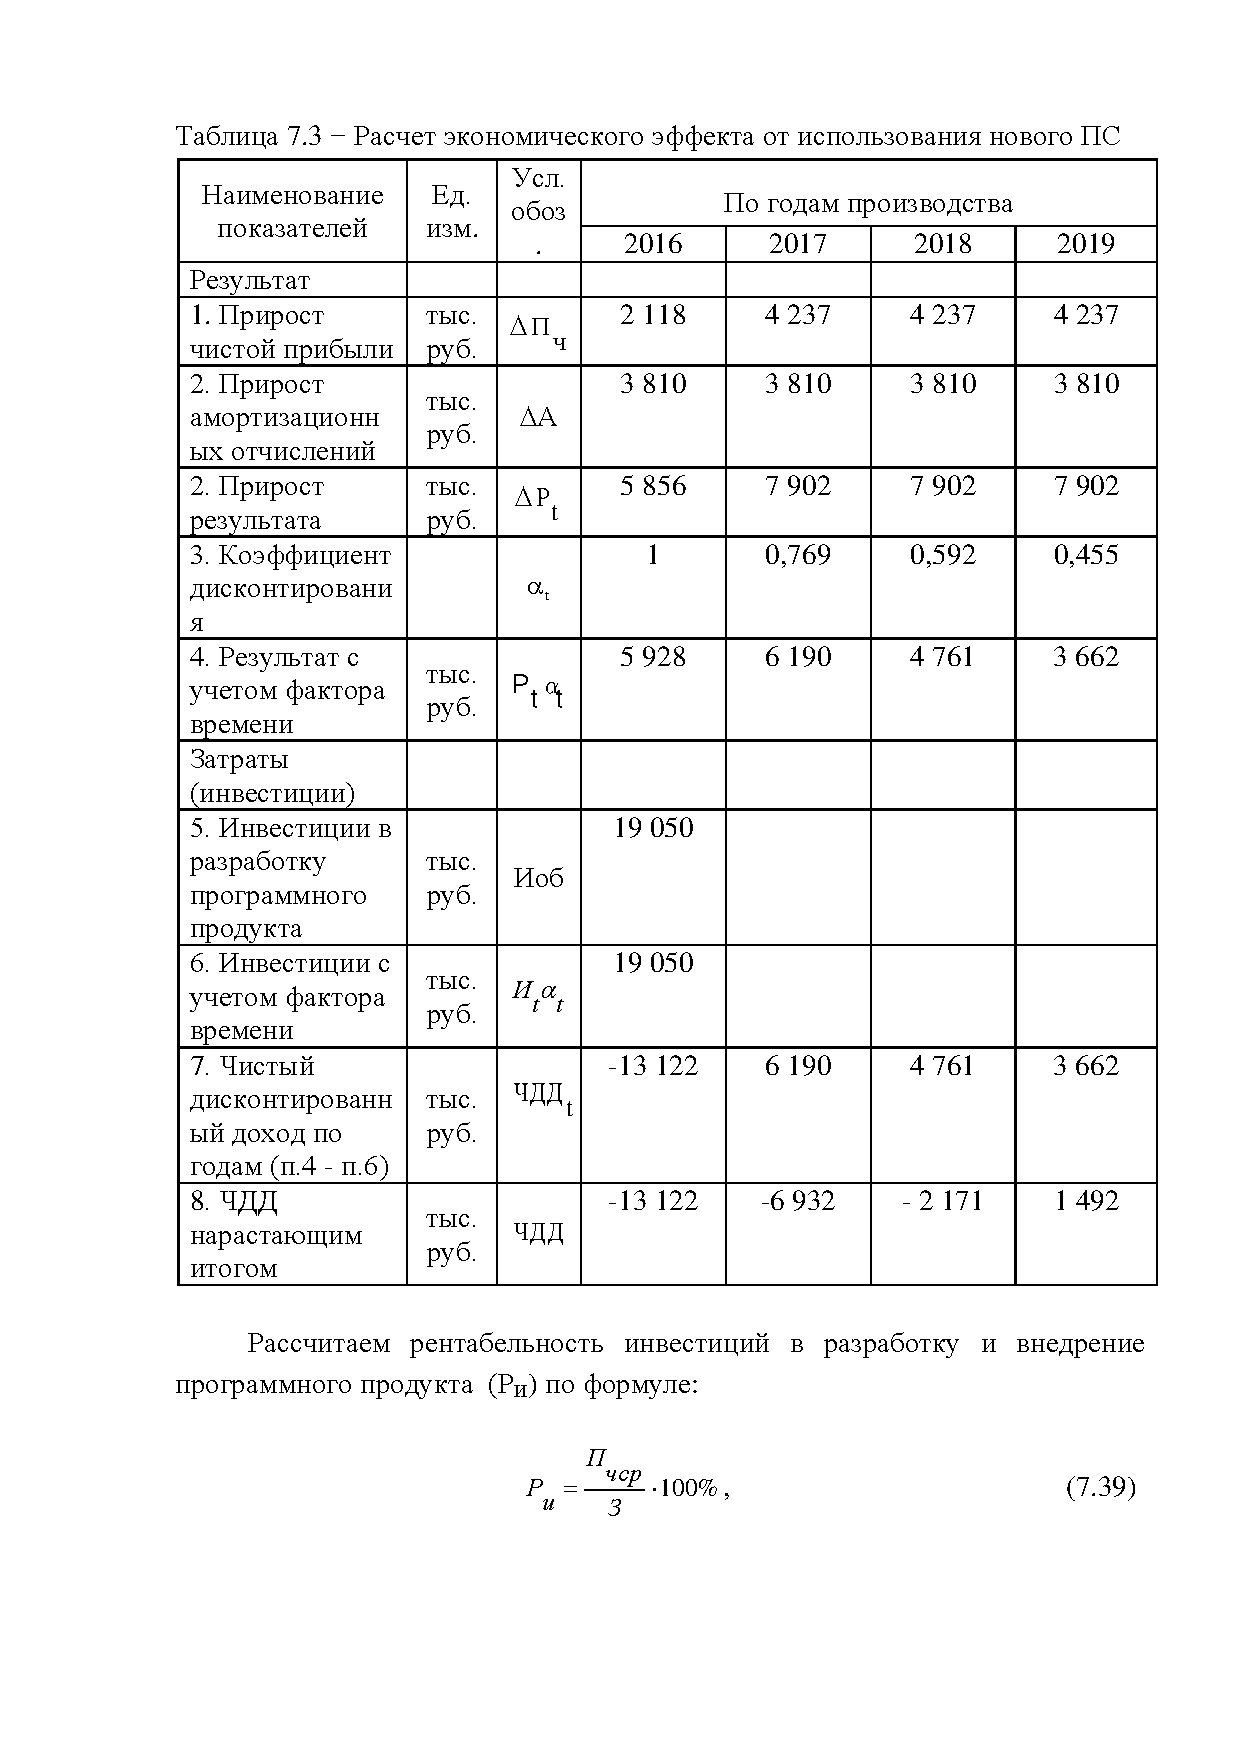
\includepdf[pages={-}, pagecommand={}]{economic_table.pdf}

% Учитывая срок разработки проекта $ \text{Т}_\text{р} = \SI{\developmentTimeMonths}{\text{мес.}} = \SI{\developmentTimeYears}{\text{года}} $, общую трудоемкость и фонд эффективного времени одного работника, вычисленные ранее, можем рассчитать численность исполнителей проекта
% \begin{equation}
%   \label{eq:econ:num_of_programmers_calc}
%   \text{Ч}_\text{р} = 
%     \frac{\num{\adjustedManDays}}
%          {\num{\developmentTimeYears} \times \num{\workingDaysInYear}} 
%     \approx \SI{\requiredNumberOfProgrammers}{\text{рабочих}}.
% \end{equation}

% Вычисленные оценки показывают, что для выполнения запланированного проекта в указанные сроки необходимо два рабочих.
% Информация о работниках перечислена в таблице~\ref{table:econ:programmers}.
% \begin{table}[ht]
%   \caption{Работники, занятые в проекте}
%   \label{table:econ:programmers}
%   \begin{tabular}{| >{\centering}m{0.4\textwidth} 
%                   | >{\centering}m{0.15\textwidth} 
%                   | >{\centering}m{0.18\textwidth} 
%                   | >{\centering\arraybackslash}m{0.15\textwidth}|}
%    \hline
%    Исполнители & Разряд & Тарифный коэффициент & \mbox{Чел./дн.} занятости \\
%    \hline
%    Программист \Rmnum{1}-категории & $ \num{13} $ & $ \num{\tariffFactorFst} $ & $ \num{\employmentFst} $ \\
%    \hline
%    Ведущий программист & $ \num{15} $ & $ \num{\tariffFactorSnd} $ & $ \num{\employmentSnd} $ \\
%    \hline
%   \end{tabular}
% \end{table}

% Месячная тарифная ставка одного работника вычисляется по формуле
% \begin{equation}
%   \label{eq:econ:month_salary}
%   \text{Т}_\text{ч} = 
%     \frac {\text{Т}_{\text{м}_{1}} \cdot \text{Т}_{\text{к}} } 
%           {\text{Ф}_{\text{р}} }  \text{\,,}
% \end{equation}
% \begin{explanation}
% где & $ \text{Т}_{\text{м}_{1}} $ & месячная тарифная ставка 1-го разряда, \byr; \\
%     & $ \text{Т}_{\text{к}} $ & тарифный коэффициент, соответствующий установленному тарифному разряду; \\
%     & $ \text{Ф}_{\text{р}} $ & среднемесячная норма рабочего времени, час.
% \end{explanation}




% Подставив данные из таблицы~\ref{table:econ:programmers} в формулу~(\ref{eq:econ:month_salary}), приняв значение тарифной ставки 1-го разряда $ \text{Т}_{\text{м}_{1}} = \SI{\tariffRateFirst}{\text{\byr}} $ и среднемесячную норму рабочего времени $ \text{Ф}_{\text{р}} = \SI{\workingHoursInMonth}{\text{часов}} $ получаем
% \begin{equation}
%   \label{eq:econ:month_salary_calc1}
%   \text{Т}_{\text{ч}}^{\text{прогр. \Rmnum{1}-разр.}} = \frac{ \num{\tariffRateFirst} \times \num{\tariffFactorFst} } { \num{\workingHoursInMonth} } = \SI{\salaryPerHourFst}{\text{\byr}/\text{час;}}
% \end{equation}
% \begin{equation}
%   \label{eq:econ:month_salary_calc2}
%   \text{Т}_{\text{ч}}^{\text{вед. прогр.}} = \frac{ \num{\tariffRateFirst} \times \num{\tariffFactorSnd} } { \num{\workingHoursInMonth} } = \SI{\salaryPerHourSnd}{\text{\byr}/\text{час.}}
% \end{equation}

% Основная заработная плата исполнителей на конкретное ПО рассчитывается по формуле 
% \begin{equation}
%   \label{eq:econ:total_salary}
%   \text{З}_{\text{о}} = \sum^{n}_{i = 1} 
%                         \text{Т}_{\text{ч}}^{i} \cdot
%                         \text{Т}_{\text{ч}} \cdot
%                         \text{Ф}_{\text{п}} \cdot
%                         \text{К}
%                           \text{\,,}
% \end{equation}
% \begin{explanation}
% где & $ \text{Т}_{\text{ч}}^{i} $ & часовая тарифная ставка \mbox{$ i $-го} исполнителя, \byr$/$час; \\
%     & $ \text{Т}_{\text{ч}} $ & количество часов работы в день, час; \\
%     & $ \text{Ф}_{\text{п}} $ & плановый фонд рабочего времени \mbox{$ i $-го} исполнителя, дн.; \\
%     & $ \text{К} $ & коэффициент премирования.
% \end{explanation}

% Подставив ранее вычисленные значения и данные из таблицы~\ref{table:econ:programmers} в формулу~(\ref{eq:econ:total_salary}) и приняв коэффициент премирования $ \text{К} = \num{\bonusRate} $ получим
% \begin{equation}
%   \label{eq:econ:total_salary_calc}
%   \text{З}_{\text{о}} = (\salaryPerHourFst \times \num{\employmentFst} + \salaryPerHourSnd \times \num{\employmentSnd}) \times \num{\workingHoursInDay} \times \num{\bonusRate} = \SI{\totalSalary}{\text{\byr}} \text{\,.}
% \end{equation}

% Дополнительная заработная плата включает выплаты предусмотренные законодательством от труде и определяется по нормативу в процентах от основной заработной платы
% \begin{equation}
%   \label{eq:econ:additional_salary}
%   \text{З}_{\text{д}} = 
%     \frac {\text{З}_{\text{о}} \cdot \text{Н}_{\text{д}}} 
%           {100\%} \text{\,,}
% \end{equation}
% \begin{explanation}
%   где & $ \text{Н}_{\text{д}} $ & норматив дополнительной заработной платы, $ \% $.
% \end{explanation}

% Приняв норматив дополнительной заработной платы $ \text{Н}_{\text{д}} = \num{\additionalSalaryNormative\%} $ и подставив известные данные в формулу~(\ref{eq:econ:additional_salary}) получим
% \begin{equation}
%   \label{eq:econ:additional_salary_calc}
%   \text{З}_{\text{д}} = 
%     \frac{\num{\totalSalary} \times 20\%}
%          {100\%} \approx \SI{\additionalSalary}{\text{\byr}} \text{\,.}
% \end{equation}

% Согласно действующему законодательству отчисления в фонд социальной защиты населения составляют \num{\socialProtectionNormative\%} , в фонд обязательного страхования "--- \num{\socialNeedsNormative\%}, от фонда основной и дополнительной заработной платы исполнителей.
% Общие отчисления на социальную защиту рассчитываются по формуле
% \begin{equation}
%   \label{eq:econ:soc_prot}
%   \text{З}_{\text{сз}} = 
%     \frac{(\text{З}_{\text{о}} + \text{З}_{\text{д}}) \cdot \text{Н}_{\text{сз}}}
%          {\num{100\%}} \text{\,.}
% \end{equation}

% Подставив вычисленные ранее значения в формулу~(\ref{eq:econ:soc_prot}) получаем
% \begin{equation}
%   \label{eq:econ:soc_prot_calc}
%   \text{З}_{\text{сз}} =
%     \frac{ (\num{\totalSalary} + \num{\additionalSalary}) \times \num{\socialProtectionFund\%} }
%          { \num{100\%} }
%     \approx \SI{\socialProtectionCost}{\text{\byr}} \text{\,.}
% \end{equation}

% \begin{comment}
%   Расчет налогов от фонда оплаты труда производится формуле
%   \begin{equation}
%     \label{eq:econ:tax_work_prot}
%     \text{Н}_{\text{е}} = 
%       \frac{(\text{З}_{\text{о}} + \text{З}_{\text{д}}) \cdot \text{Н}_{\text{не}}}
%            {\num{100\%}} \text{\,,}
%   \end{equation}
%   \begin{explanation}
%     где & $ \text{Н}_{\text{не}} $ & норматив налога, уплачиваемый единым платежом, $ \% $.
%   \end{explanation}

%   Подставив ранее вычисленные значения в формулу~(\ref{eq:econ:tax_work_prot}) и приняв норматив налога $ \text{Н}_{\text{не}} = \num{\taxWorkProtNormative\%} $ получаем
%   \begin{equation}
%     \label{eq:econ:tax_work_prot_calc}
%     \text{Н}_{\text{е}} = 
%         \frac{ (\num{\totalSalary} + \num{\additionalSalary}) \times \num{\taxWorkProtNormative\%} }
%            { \num{100\%} }
%       \approx \SI{\taxWorkProtCost}{\text{\byr}}\text{\,.}
%   \end{equation}
% \end{comment}

% По статье <<материалы>> проходят расходы на носители информации, бумагу, краску для принтеров и другие материалы, используемые при разработке ПО.
% Норма расходов $ \text{Н}_{\text{мз}} $ определяется либо в расчете на \num{100} строк исходного кода, либо в процентах к основной зарплате исполнителей \mbox{\num{3\%}\,---\,\num{5\%}}.
% Затраты на материалы вычисляются по формуле
% \begin{equation}
%   \label{eq:econ:stuff}
%   \text{М} = 
%     \frac{ \text{З}_{\text{о}} \cdot \text{Н}_{\text{мз}} }
%          { \num{100\%} } =
%     \frac{ \num{\totalSalary} \times \num{\stuffNormative\%} }
%          { \num{100\%} } \approx
%     \SI{\stuffCost}{\text{\byr}} \text{\,.}
% \end{equation}

% Расходы по статье <<машинное время>> включают оплату машинного времени, необходимого для разработки и отладки ПО, которое определяется по нормативам в машино-часах на \num{100} строк исходного кода в зависимости от характера решаемых задач и типа ПК, и вычисляются по формуле
% \begin{equation}
%   \label{eq:econ:machine_time}
%   \text{Р}_{\text{м}} =
%     \text{Ц}_{\text{м}} \cdot 
%     \frac {\text{V}_{\text{о}}}
%           {\num{100}} \cdot
%     \text{Н}_{\text{мв}} \text{\,,}
% \end{equation}
% \begin{explanation}
%   где & $ \text{Ц}_{\text{м}} $ & цена одного часа машинного времени, \byr; \\
%       & $ \text{Н}_{\text{мв}} $ & норматив расхода машинного времени на отладку 100 строк исходного кода, часов.
% \end{explanation}

% Согласно нормативу~\cite[с.\,69, приложениe~6]{palicyn_2006} норматив расхода машинного времени на отладку \num{100} строк исходного кода составляет $ \text{Н}_{\text{мв}} = \num{\timeToDebugCodeNormative} $, применяя понижающий коэффициент \num{\reducingTimeToDebugFactor} получаем $ {\text{Н}'}_{\text{мв}} = \num{\adjustedTimeToDebugCodeNormative} $.
% Цена одного часа машинного времени составляет $ \text{Ц}_{\text{м}} = \SI{\oneHourMachineTimeCost}{\text{\byr}} $.
% Подставляя известные данные в формулу~(\ref{eq:econ:machine_time}) получаем
% \begin{equation}
%   \label{eq:econ:machine_time_calc}
%   \text{Р}_{\text{м}} =
%     \num{\oneHourMachineTimeCost} \times 
%     \frac {\num{\totalProgramSizeCorrected}}
%           {\num{100}} \times
%     \num{\adjustedTimeToDebugCodeNormative} =
%     \SI{\machineTimeCost}{\text{\byr}} \text{\,.}
% \end{equation}

% Расходы по статье <<научные командировки>> вычисляются как процент от основной заработной платы, либо определяются по нормативу. 
% Вычисления производятся по формуле
% \begin{equation}
%   \label{eq:econ:business_trip}
%   \text{Р}_{\text{к}} =
%     \frac{ \text{З}_{\text{о}} \cdot \text{Н}_{\text{к}} }
%          { \num{100\%} } \text{\,,}
% \end{equation}
% \begin{explanation}
%   где & $ \text{Н}_{\text{к}} $ & норматив командировочных расходов по отношению к основной заработной плате, $ \% $.
% \end{explanation}

% Подставляя ранее вычисленные значения в формулу~(\ref{eq:econ:business_trip}) и приняв значение $ \text{Н}_{\text{к}} = \num{\businessTripNormative\%} $ получаем
% \begin{equation}
%   \label{eq:econ:business_trip_calc}
%     \text{Р}_{\text{к}} =
%     \frac{ \num{\totalSalary} \times \num{\businessTripNormative\%} }
%          { \num{100\%} } = \SI{\businessTripCost}{\text{\byr}} \text{\,.}
% \end{equation}

% Статья расходов <<прочие затраты>> включает в себя расходы на приобретение и подготовку специальной научно-технической информации и специальной литературы.
% Затраты определяются по нормативу принятому в организации в процентах от основной заработной платы и вычисляются по формуле
% \begin{equation}
%   \label{eq:econ:other_cost}
%   \text{П}_{\text{з}} =
%     \frac{ \text{З}_{\text{о}} \cdot \text{Н}_{\text{пз}} }
%          { \num{100\%} } \text{\,,}
% \end{equation}
% \begin{explanation}
%   где & $ \text{Н}_{\text{пз}} $ & норматив прочих затрат в целом по организации, $ \% $.
% \end{explanation}

% Приняв значение норматива прочих затрат $ \text{Н}_{\text{пз}} = \num{\otherCostNormative\%} $ и подставив вычисленные ранее значения в формулу~(\ref{eq:econ:other_cost}) получаем
% \begin{equation}
%   \label{eq:econ:other_cost_calc}
%   \text{П}_{\text{з}} =
%     \frac{ \num{\totalSalary} \times \num{\otherCostNormative\%} }
%          { \num{100\%} } = 
%     \SI{\otherCost}{\text{\byr}} \text{\,.}
% \end{equation}

% Статья <<накладные расходы>> учитывает расходы, необходимые для содержания аппарата управления, вспомогательных хозяйств и опытных производств, а также расходы на общехозяйственные нужны. Данная статья затрат рассчитывается по нормативу от основной заработной платы и вычисляется по формуле.

% \begin{equation}
%   \label{eq:econ:overhead_cost}
%   \text{Р}_{\text{н}} =
%     \frac{ \text{З}_{\text{о}} \cdot \text{Н}_{\text{рн}} }
%          { \num{100\%} } \text{\,,}
% \end{equation}
% \begin{explanation}
%   где & $ \text{Н}_{\text{рн}} $ & норматив накладных расходов в организации,~$ \% $.
% \end{explanation}

% Приняв норму накладных расходов $ \text{Н}_{\text{рн}} = \num{\overheadCostNormative\%} $ и подставив известные данные в формулу~(\ref{eq:econ:overhead_cost}) получаем
% \begin{equation}
%   \label{eq:econ:overhead_cost_calc}
%   \text{Р}_{\text{н}} =
%     \frac{ \num{\totalSalary} \times \num{\overheadCostNormative\%} }
%          { \num{100\%} } = 
%     \SI{\overheadCost}{\text{\byr}} \text{\,.}
% \end{equation}

% Общая сумма расходов по смете на ПО рассчитывается по формуле
% \begin{equation}
%   \label{eq:econ:overall_cost}
%   \text{С}_{\text{р}} =
%     \text{З}_{\text{о}} +
%     \text{З}_{\text{д}} +
%     \text{З}_{\text{сз}} +
%     %\text{Н}_{\text{е}} +
%     \text{М} +
%     % \text{Р}_{\text{с}} + % спецоборудование не нужно
%     \text{Р}_{\text{м}} +
%     \text{Р}_{\text{нк}} +
%     \text{П}_{\text{з}} +
%     \text{Р}_{\text{н}}\text{\,.}
% \end{equation}

% Подставляя ранее вычисленные значения в формулу~(\ref{eq:econ:overall_cost}) получаем

% \begin{equation}
%   \label{eq:econ:overall_cost_calc}
%   \text{С}_{\text{р}} = \SI{\overallCost}{\text{\byr}} \text{\,.}
% \end{equation}

% Расходы на сопровождение и адаптацию, которые несет производитель ПО, вычисляются по нормативу от суммы расходов по смете и рассчитываются по формуле
% \begin{equation}
%   \label{eq:econ:software_support}
%   \text{Р}_{\text{са}} = 
%     \frac { \text{С}_{\text{р}} \cdot \text{Н}_{\text{рса}} }
%           { \num{100\%} } \text{\,,}
% \end{equation}
% \begin{explanation}
%   где & $ \text{Н}_{\text{рса}} $ & норматив расходов на сопровождение и адаптацию ПО,~$ \% $.
% \end{explanation}

% Приняв значение норматива расходов на сопровождение и адаптацию $ \text{Н}_{\text{рса}} = \num{\supportNormative\%} $ и подставив ранее вычисленные значения в формулу~(\ref{eq:econ:software_support}) получаем
% \begin{equation}
%   \label{eq:econ:software_support_calc}
%   \text{Р}_{\text{са}} = 
%     \frac { \num{\overallCost} \times \num{\supportNormative\%} }
%           { \num{100\%} } \approx \SI{\softwareSupportCost}{\text{\byr}} \text{\,.}
% \end{equation}

% Полная себестоимость создания ПО включает сумму затрат на разработку, сопровождение и адаптацию и вычисляется по формуле
% \begin{equation}
%   \label{eq:econ:base_cost}
%   \text{С}_{\text{п}} = \text{С}_{\text{р}} + \text{Р}_{\text{са}} \text{\,.}
% \end{equation}

% Подставляя известные значения в формулу~(\ref{eq:econ:base_cost}) получаем
% \begin{equation}
%   \label{eq:econ:base_cost_calc}
%   \text{С}_{\text{п}} = \num{\overallCost} + \num{\softwareSupportCost} = \SI{\baseCost}{\text{\byr}} \text{\,.}
% \end{equation}



% \subsection{Расчёт экономической эффективности у разработчика}

% Важная задача при выборе проекта для финансирования это расчет экономической эффективности проектов и выбор наиболее выгодного проекта.
% \begin{comment}
%   Оценка коммерческой эффективности проектов ПО предполагает:
%   \begin{itemize}
%     \item определение расчётного периода и расчётных шагов проекта; 
%     \item обоснование цены ПО;
%     \item определение денежных потоков с включением всех денежных поступлений по проекту в ходе его осуществления; 
%     \item учёт изменения стоимости денег во времени;
%     \item оценку затрат и результатов по проекту в соответствии с  принципом <<без проекта>> и <<с проектом>>; 
%     \item оценку инфляции и риска;
%     \item учёт налогов, сборов, отчислений и льгот, предусмотренных законодательными нормами, действующими в расчётном периоде.
%   \end{itemize}
% \end{comment}
% Разрабатываемое ПО является заказным, т.\,е.~разрабатывается для одного заказчика на заказ.
% На основании анализа рыночных условий и договоренности с заказчиком об отпускной цене прогнозируемая рентабельность проекта составит~$ \text{У}_{\text{рп}} = \num{\profitability\%} $.
% Прибыль рассчитывается по формуле
% \begin{equation}
%   \label{eq:econ:income}
%   \text{П}_{\text{с}} = 
%     \frac { \text{С}_{\text{п}} \cdot \text{У}_{\text{рп}} }
%           { \num{100\%} } \text{\,,}
% \end{equation}
% \begin{explanation}
%   где & $ \text{П}_{\text{с}} $ & прибыль от реализации ПО заказчику, \byr; \\
%       & $ \text{У}_{\text{рп}} $ & уровень рентабельности ПО,~$ \% $.
% \end{explanation}

% Подставив известные данные в формулу~(\ref{eq:econ:income}) получаем прогнозируемую прибыль от реализации ПО
% \begin{equation}
%   \label{eq:econ:income_calc}
%   \text{П}_{\text{с}} = 
%     \frac { \num{\baseCost} \times \num{\profitability\%} }
%           { \num{100\%} } 
%     \approx \SI{\income}{\text{\byr}} \text{\,.}
% \end{equation}

% Прогнозируемая цена ПО без учета налогов включаемых в цену вычисляется по формуле 
% \begin{equation}
%   \label{eq:econ:estimated_price}
%   \text{Ц}_{\text{п}} = \text{С}_{\text{п}} + \text{П}_{\text{с}}  \text{\,.}
% \end{equation}

% Подставив данные в формулу~(\ref{eq:econ:estimated_price}) получаем цену ПО без налогов
% \begin{equation}
%   \label{eq:econ:estimated_price_calc}
%   \text{Ц}_{\text{п}} = \num{\baseCost}  + \num{\income} = \SI{\estimatedPrice}{\text{\byr}} \text{\,.}
% \end{equation}

% \begin{comment}
%   Отчисления и налоги в местный и республиканский бюджеты вычисляются по формуле
%   \begin{equation}
%     \label{eq:econ:local_repub_tax}
%     \text{О}_{\text{мр}} =
%       \frac { \text{Ц}_{\text{п}} \cdot \text{Н}_{\text{мр}} }
%             { \num{100\%} - \text{Н}_{\text{мр}} } \text{\,,}
%   \end{equation}
%   \begin{explanation}
%     где & $ \text{Н}_{\text{мр}} $ & норматив отчислений в местный и республиканский бюджеты, \byr.
%   \end{explanation}

%   Приняв норматив отчислений в местный и республиканский бюджеты $ \text{Н}_{\text{мр}} = \num{\localRepubTaxNormative\%} $ и подставив известные данные в формулу~(\ref{eq:econ:local_repub_tax}) получим величину единого платежа
%   \begin{equation}
%     \label{eq:econ:local_repub_tax_calc}
%     \text{О}_{\text{мр}} = 
%       \frac { \num{\estimatedPrice} \cdot \num{\localRepubTaxNormative\%} }
%             { \num{100\%} - \num{\localRepubTaxNormative\%} } 
%       \approx \SI{\localRepubTax}{\text{\byr}} \text{\,.}
%   \end{equation}
% \end{comment}

% Налог на добавленную стоимость рассчитывается по формуле
% \begin{equation}
%   \label{eq:econ:nds}
%   \text{НДС}_{\text{}} =
%     \frac{ \text{Ц}_{\text{п}} \cdot \text{Н}_{\text{дс}} }
%          { \num{100\%} } \text{\,,}
% \end{equation}
% \begin{explanation}
%   где & $ \text{Н}_{\text{дс}} $ & норматив НДС,~$\%$.
% \end{explanation}

% Норматив НДС составляет $ \text{Н}_{\text{дс}} = \num{\ndsNormative\%} $, подставляя известные значения в формулу~(\ref{eq:econ:nds}) получаем
% \begin{equation}
%   \text{НДС} =
%     \frac { \num{\estimatedPrice} \times \num{\ndsNormative\%} }
%           { \num{100\% }} 
%     \approx \SI{\nds}{\text{\byr}} \text{\,.}
% \end{equation}

% Расчет прогнозируемой отпускной цены осуществляется по формуле 
% \begin{equation}
%   \label{eq:econ:selling_price}
%   \text{Ц}_{\text{о}} = \text{Ц}_{\text{п}} + \text{НДС} \text{\,.}
% \end{equation}

% Подставляя известные данные в формулу~(\ref{eq:econ:selling_price}) получаем прогнозируемую отпускную цену
% \begin{equation}
%   \label{eq:econ:selling_price_calc}
%   \text{Ц}_{\text{о}} = \num{\estimatedPrice} + \num{\nds} \approx \SI{\sellingPrice}{\text{\byr}} \text{\,.}
% \end{equation}


% Чистую прибыль от реализации проекта можно рассчитать по формуле
% \begin{equation}
%   \label{eq:econ:income_with_taxes}
%   \text{П}_\text{ч} = 
%     \text{П}_\text{c} \cdot
%     \left(1 - \frac{ \text{Н}_\text{п} }{ \num{100\%} } \right) \text{\,,}
% \end{equation}
% \begin{explanation}
%   где & $ \text{Н}_{\text{п}} $ & величина налога на прибыль,~$\%$.
% \end{explanation}

% Приняв значение налога на прибыль $ \text{Н}_{\text{н}} = \num{\taxForIncome\%} $ и подставив известные данные в формулу~(\ref{eq:econ:income_with_taxes}) получаем чистую прибыль
% \begin{equation}
%   \label{eq:econ:income_with_taxes_calc}
%   \text{П}_\text{ч} = 
%     \num{\income} \times \left( 1 - \frac{\num{\taxForIncome\%}}{100\%} \right) = \SI{\incomeWithTaxes}{\text{\byr}} \text{\,.}
% \end{equation}

% Программное обеспечение разрабатывалось для одного заказчика в связи с этим экономическим эффектом разработчика будет являться чистая прибыль от реализации~$ \text{П}_\text{ч} $.
% Рассчитанные данные приведены в таблице~\ref{table:econ:calculated_data}.
% Таким образом было произведено технико"=экономическое обоснование разрабатываемого проекта, составлена смета затрат и рассчитана прогнозируемая прибыль, и показана экономическая целесообразность разработки.

% \begin{table}[!h!t]
% \caption{Рассчитанные данные}
% \label{table:econ:calculated_data}
%   \centering
%   \begin{tabular}{| >{\raggedright}m{0.60\textwidth} 
%                   | >{\centering}m{0.17\textwidth} 
%                   | >{\centering\arraybackslash}m{0.15\textwidth}|}
%     \hline
%     {\begin{center}
%       Наименование
%     \end{center} } & Условное обозначение & Значение \\
%     \hline
%     Нормативная трудоемкость, чел.$/$дн. & $ \text{Т}_\text{н} $ & \num{\normativeManDays} \\

%     \hline
%     Общая трудоемкость разработки, чел.$/$дн. & $ \text{Т}_\text{о} $ & \num{\adjustedManDays} \\

%     \hline
%     Численность исполнителей, чел. & $ \text{Ч}_\text{р} $ & \num{\requiredNumberOfProgrammers} \\

%     \hline
%     Часовая тарифная ставка программиста \Rmnum{1}-разряда, \byr{}$/$ч. & $ \text{Т}_{\text{ч}}^{\text{прогр. \Rmnum{1}-разр.}} $ & \num{\salaryPerHourFst} \\

%     \hline
%     Часовая тарифная ставка ведущего программиста, \byr{}$/$ч. & $ \text{Т}_{\text{ч}}^{\text{вед. прогр.}} $ & \num{\salaryPerHourSnd} \\

%     \hline
%     Основная заработная плата, \byr{} & $ \text{З}_\text{о} $ & \num{\totalSalary} \\

%     \hline
%     Дополнительная заработная плата, \byr{} & $ \text{З}_\text{д}$ & \num{\additionalSalary} \\

%     \hline
%     Отчисления в фонд социальной защиты, \byr{} & $ \text{З}_\text{сз} $ & \num{\socialProtectionCost} \\

%     \hline
%     Затраты на материалы, \byr{} & $ \text{М} $ & \num{\stuffCost} \\

%     \hline
%     Расходы на машинное время, \byr{} & $ \text{Р}_\text{м} $ & \num{\machineTimeCost} \\

%     \hline
%     Расходы на командировки, \byr{} & $ \text{Р}_\text{к} $ & \num{\businessTripCost} \\

%     \hline
%     Прочие затраты, \byr{} & $ \text{П}_\text{з} $ & \num{\otherCost} \\

%     \hline
%     Накладные расходы, \byr{} & $ \text{Р}_\text{н} $ & \num{\overheadCost} \\

%     \hline
%     Общая сумма расходов по смете, \byr{} & $ \text{С}_\text{р} $ & \num{\overallCost} \\

%     \hline
%     Расходы на сопровождение и адаптацию, \byr{} & $ \text{Р}_\text{са} $ & \num{\softwareSupportCost} \\

%     \hline
%     Полная себестоимость, \byr{} & $ \text{С}_\text{п} $ & \num{\baseCost} \\

%     \hline
%     Прогнозируемая прибыль, \byr{} & $ \text{П}_\text{с} $ & \num{\income} \\

%     \hline
%     НДС, \byr{} & $ \text{НДС} $ & \num{\nds} \\

%     \hline
%     Прогнозируемая отпускная цена ПО, \byr{} & $ \text{Ц}_\text{о} $ & \num{\sellingPrice} \\

%     \hline
%     Чистая прибыль, \byr{} & $ \text{П}_\text{ч} $ & \num{\incomeWithTaxes} \\

%     \hline
%   \end{tabular}
% \end{table}
% \hfill
% \clearpage


% % Часть, которая, к сожалению, была написана, наверное, зря.
% \begin{comment}

% Договоренность с заказчиком предусматривает оплату за ПО после его адаптации на стороне заказчика. 
% Следствием из данной договоренности являются возникающие риски для организации исполнителя связанные с неуплатой стоимости проекта заказчиком.
% На случай провала сделки с определенным заказчиком рассмотрим бизнес"=план, который предусматривает массовую реализацию разрабатываемого ПО по сниженной цене, и оценим экономическую эффективность разработки с данной точки зрения.

% \FPeval{\priceFirstYear}{1500}
% \FPeval{\priceSecondYear}{1250}
% \FPeval{\priceThirdYear}{1000}
% Расчетный период для разрабатываемого проекта состоит из трех интервалов времени длительностью один год. 
% На рынке существует достаточное количество как платных так и бесплатных аналогов разрабатываемого продукта. Анализ платных продуктов показал, что начальную цену на одну лицензию целесообразно установить ниже средней на рынке в размере $ P_1 = \SI{\priceFirstYear}{\text{тыс.\,\byr}} $, в последующие отрезки времени расчетного периода $ t_2 $ и $ t_3 $ планируется планомерно снижать цену до $ P_2 = \SI{\priceSecondYear}{\text{тыс.\,\byr}} $ и $ P_3 = \SI{\priceThirdYear}{\text{тыс.\,\byr}} $ для привлечения новых клиентов.

% \FPeval{\soldInFirstYear}{30}
% \FPeval{\soldInSecondYear}{50}
% \FPeval{\soldInThirdYear}{40}
% В связи с тем, что разрабатываемое ПО не предназначено для широкого круга пользователей, то прогнозируемый уровень продаж для расчетного периода составит $ Q_1 = \num{\soldInFirstYear} $, $ Q_2 = \num{\soldInSecondYear} $ и $ Q_3 = \num{\soldInThirdYear} $ копий.

% \FPeval{\revenueInFirstYear}{clip(\soldInFirstYear * \priceFirstYear)}
% \FPeval{\revenueInSecondYear}{clip(\soldInSecondYear * \priceSecondYear)}
% \FPeval{\revenueInThirdYear}{clip(\soldInThirdYear * \priceThirdYear)}
% Выручка от продаж в $i$-й отрезок времени расчетного периода вычисляется по формуле
% \begin{equation}
%   \label{eq:econ:profit}
%   \text{Д}^\text{р}_i = P_i \cdot Q_i \text{\,.}
% \end{equation}

% Рассчитанные данные приведены в таблице~\ref{table:econ:justification}. Входной денежный поток в $i$-й отрезок времени расчетного периода рассчитывается по формуле
% \begin{equation}
%   \label{eq:econ:income_cash_flow}
%   \text{ДП}^\text{п}_i = \text{Д}^\text{р}_i + \text{А}^\text{о}_i \text{\,.}
% \end{equation}
% \begin{explanation}
% где & $ \text{А}^\text{о}_i $ & амортизационные отчисления, \byr.
% \end{explanation}

% \FPeval{\depreciations}{3000}
% \FPeval{\firstYearCashFlowIncome}{clip(\depreciations + \revenueInFirstYear)}
% \FPeval{\secondYearCashFlowIncome}{clip(\depreciations + \revenueInSecondYear)}
% \FPeval{\thirdYearCashFlowIncome}{clip(\depreciations + \revenueInThirdYear)}

% Выходной денежный поток рассчитывается в $i$-й отрезок времени расчетного периода вычисляется по формуле
% \begin{equation}
%   \label{eq:econ:cash_flow_outcome}
%   \text{ДП}^\text{о}_i = \text{Р}^\text{п}_i + \text{Р}^\text{у}_i + \text{Р}^\text{н}_i
% \end{equation}
% \begin{explanation}
% где & $ \text{Р}^\text{п}_i $ & переменные затраты на производство и реализацию, \byr; \\
%     & $ \text{Р}^\text{у}_i $ & расходы постоянные на управление и обслуживание, \byr; \\
%     & $ \text{Р}^\text{н}_i $ & налоги, уплачиваемые из прибыли.
% \end{explanation}

% Прогнозируемые постоянные и переменные затраты, а также налоги и выходные денежные потоки приведены в таблице~\ref{table:econ:justification}. Норматив налога на прибыль принят $ \text{Н}_\text{нп} = \num{12\%} $. 

\FPeval{\firstYearVariableCosts}{17200}
\FPeval{\secondYearVariableCosts}{18300}
\FPeval{\thirdYearVariableCosts}{15800}

\FPeval{\firstYearConstCosts}{12000}
\FPeval{\secondYearConstCosts}{11100}
\FPeval{\thirdYearConstCosts}{9400}

\FPeval{\firstYearCostOfProduction}{clip(\firstYearVariableCosts + \firstYearConstCosts)}
\FPeval{\secondYearCostOfProduction}{clip(\secondYearVariableCosts + \secondYearConstCosts)}
\FPeval{\thirdYearCostOfProduction}{clip(\thirdYearVariableCosts + \thirdYearConstCosts)}

\FPeval{\firstYearGrossProfit}{clip(\revenueInFirstYear - \firstYearCostOfProduction)}
\FPeval{\secondYearGrossProfit}{clip(\revenueInSecondYear - \secondYearCostOfProduction)}
\FPeval{\thirdYearGrossProfit}{clip(\revenueInThirdYear - \thirdYearCostOfProduction)}

\FPeval{\firstYearPropertyTax}{300}
\FPeval{\secondYearPropertyTax}{300}
\FPeval{\thirdYearPropertyTax}{300}

\FPeval{\firstYearTaxableIncome}{clip(\firstYearGrossProfit - \firstYearPropertyTax)}
\FPeval{\secondYearTaxableIncome}{clip(\secondYearGrossProfit - \secondYearPropertyTax)}
\FPeval{\thirdYearTaxableIncome}{clip(\thirdYearGrossProfit - \thirdYearPropertyTax)}

\FPeval{\incomeTax}{0.12}
\FPeval{\fyIncomeTax}{clip(\firstYearTaxableIncome * \incomeTax)}
\FPeval{\syIncomeTax}{clip(\secondYearTaxableIncome * \incomeTax)}
\FPeval{\tyIncomeTax}{clip(\thirdYearTaxableIncome * \incomeTax)}

\FPeval{\fyNetIncome}{clip(\firstYearTaxableIncome - \fyIncomeTax)}
\FPeval{\syNetIncome}{clip(\secondYearTaxableIncome - \syIncomeTax)}
\FPeval{\tyNetIncome}{clip(\thirdYearTaxableIncome - \tyIncomeTax)}

\FPeval{\capitalInvestments}{clip(\baseCost / 1000)}
\FPround\capitalInvestments{\capitalInvestments}{0}

\FPeval{\discountRate}{0.295}

\FPeval{\zyDiscountFactor}{1}
\FPeval{\fyDiscountFactor}{clip(\zyDiscountFactor / (1 + \discountRate))}
\FPeval{\syDiscountFactor}{clip(\fyDiscountFactor / (1 + \discountRate))}
\FPeval{\tyDiscountFactor}{clip(\syDiscountFactor / (1 + \discountRate))}


\FPeval{\fyCashFlowOutcome}{clip(\firstYearCostOfProduction + \firstYearPropertyTax + \fyIncomeTax)}
\FPeval{\syCashFlowOutcome}{clip(\secondYearCostOfProduction + \secondYearPropertyTax + \syIncomeTax)}
\FPeval{\tyCashFlowOutcome}{clip(\thirdYearCostOfProduction + \thirdYearPropertyTax + \tyIncomeTax)}

\FPeval{\fyCashFlowOutcomeDiscounted}{clip(\fyCashFlowOutcome * \fyDiscountFactor)}
\FPeval{\syCashFlowOutcomeDiscounted}{clip(\syCashFlowOutcome * \syDiscountFactor)}
\FPeval{\tyCashFlowOutcomeDiscounted}{clip(\tyCashFlowOutcome * \tyDiscountFactor)}

\FPeval{\fyCashFlowIncomeDiscounted}{clip(\firstYearCashFlowIncome * \fyDiscountFactor)}
\FPeval{\syCashFlowIncomeDiscounted}{clip(\secondYearCashFlowIncome * \syDiscountFactor)}
\FPeval{\tyCashFlowIncomeDiscounted}{clip(\thirdYearCashFlowIncome * \tyDiscountFactor)}

\FPround\fyDiscountFactor{\fyDiscountFactor}{3}
\FPround\syDiscountFactor{\syDiscountFactor}{3}
\FPround\tyDiscountFactor{\tyDiscountFactor}{3}

\FPround\fyCashFlowIncomeDiscounted{\fyCashFlowIncomeDiscounted}{0}
\FPround\syCashFlowIncomeDiscounted{\syCashFlowIncomeDiscounted}{0}
\FPround\tyCashFlowIncomeDiscounted{\tyCashFlowIncomeDiscounted}{0}

\FPround\fyCashFlowOutcomeDiscounted{\fyCashFlowOutcomeDiscounted}{0}
\FPround\syCashFlowOutcomeDiscounted{\syCashFlowOutcomeDiscounted}{0}
\FPround\tyCashFlowOutcomeDiscounted{\tyCashFlowOutcomeDiscounted}{0}

\FPround\zyNetIncomeAcc{-\capitalInvestments}{0}
\FPeval{\fyNetIncomeAcc}{clip(\zyNetIncomeAcc + (\fyCashFlowIncomeDiscounted - \fyCashFlowOutcomeDiscounted))}
\FPeval{\syNetIncomeAcc}{clip(\fyNetIncomeAcc + (\syCashFlowIncomeDiscounted - \syCashFlowOutcomeDiscounted))}
\FPeval{\tyNetIncomeAcc}{clip(\syNetIncomeAcc + (\tyCashFlowIncomeDiscounted - \tyCashFlowOutcomeDiscounted))}


% Для оценки изменения стоимости денег необходимо оценить норму дисконта, которая вычисляется по формуле
% \begin{equation}
%   \label{eq:econ:discount_rate}
%   \text{Е} = r + s + \sum_{i=1}^{n} g_i \text{\,,}
% \end{equation}
% \begin{explanation}
% где & $ r $ & реальная (без учета компенсации за инфляцию) безрисковая ставка ссудного процента, \%; \\
%     & $ s $ & инфляционное ожидание за период $ t $, рассчитанное как среднее за расчетный период проекта, \%; \\
%     & $ g_i $ & премия за отдельный риск по конкретному фактору, \%.
% \end{explanation}

% Примем во внимание экономическую обстановку в Беларуси на начало 2013 года, чтобы получить значения коэффициента дисконтирования. 
% Безрисковая ставка ссудного процента составляет $r = \num{5.5\%}$, возможное влияние непредвиденных обстоятельств на величину этой ставки оценим премией за риск $ g_1 = \num{1\%} $.
% По различным данным инфляция в 2013 году в Беларуси составит $ s = \num{21\%} $. Дополнительно учтем риски падения спроса $ g_2 = \num{1\%} $ и падения дохода $ g_3 = \num{1\%}$.
% Подставляя приведенные данные в формулу~(\ref{eq:econ:discount_rate}) получаем
% \begin{equation}
%   \label{eq:econ:discount_rate_calc}
%   \text{Е} = \num{5.5\%} + \num{21\%} + \num{1\%} + \num{1\%} + \num{1\%} = \num{29.5\%} \text{\,.}
% \end{equation}

% Зная норму дисконта можно рассчитать значения коэффициентов дисконтирования для каждого из отрезков времени расчетного периода по формуле~(\ref{eq:econ:discount_factor}). Рассчитанные коэффициенты приведены в таблице~\ref{table:econ:justification}.
% \begin{equation}
%   \label{eq:econ:discount_factor}
%   \alpha_t = (1 + \text{Е})^{-t} \text{\,,}
% \end{equation}
% \begin{explanation}
% где & $ t $ & номер отрезка времени расчетного периода с момента старта проекта, \%.
% \end{explanation}

% Основным показателем экономической целесообразности реализации проекта является чистый дисконтированный доход. 
% Разрабатываемый проект предусматривает одноразовые начальные инвестиции, поэтому чистый дисконтированный доход может быть рассчитан по формуле
% \begin{equation}
%   \label{eq:econ:net_present_value}
%   \text{ЧДД} = -\text{И}_{0} + \sum_{t = 1}^m \text{ДП}^\text{п}_i \cdot \alpha_i - \sum_{t = 1}^m \text{ДП}_\text{о}^i \cdot \alpha_i \text{\,,}
% \end{equation}

% Прогнозируемые значения ЧДД приведены в таблице~\ref{table:econ:justification}. 
% Т.\,к.~значение данного экономичекого показателя $ \text{ЧДД} > 0 $, то проект приносит прибыль.
% Мы не распологаем бухгалтерскими данными по аналогичным проектам, поэтому вычисление индекса рентабельности не несет в себе полезной нагрузки и он не может быть использован для сравнения проектов.
% С финансовой точки зрения срок окупаемости проекта является спорным показателем эффективности~\cite[с.~166\,--\,167]{crundwell_2008}, по этой и по приведенной раньше причине точный расчет данного показателя производить не будем. 
% По прогнозируемым данным приведенным в таблице~\ref{table:econ:justification} приблизительный срок окупаемости проекта составит $ \text{Т}_\text{ок} \approx \SI{2}{\text{года}} $.


% \begin{table}[ht]
% \caption{Прогнозные данные реализации проекта ПО}
% \label{table:econ:justification}
% \centering
%   \begin{tabular}{| >{\raggedright}m{0.34\textwidth} 
%                   | >{\centering}m{0.091\textwidth} 
%                   | >{\centering}m{0.105\textwidth} 
%                   | >{\centering}m{0.105\textwidth} 
%                   | >{\centering}m{0.1\textwidth} 
%                   | >{\centering\arraybackslash}m{0.1\textwidth}|}
%     \hline
%       \multirow{3}{0.34\textwidth}{\centering Показатели} &
%       \multirow{3}{0.091\textwidth}{\centering Ед. измер.} &
%       \multicolumn{4}{c|}{\centering Значения показателей по шагам} \\
    
%     \cline{3-6} 
%     & & 2013 & 2014 & 2015 & 2016 \\
%     & & $ t_0 $ & $ t_1 $ & $ t_2 $ & $ t_3 $ \\
    
%     \hline
%     1 & 2 & 3 & 4 & 5 & 6 \\
    
%     \hline
%     Объём производства и реализации & штук & & \num{\soldInFirstYear} & \num{\soldInSecondYear} & \num{\soldInThirdYear} \\ 

%     \hline
%     Прогнозная рыночная цена & тыс.\,\byr & & \num{\priceFirstYear} & \num{\priceSecondYear} & \num{\priceThirdYear} \\

%     \hline
%     Выручка от продаж (без налогов, включаемых в цену) & тыс.\,\byr & & \num{\revenueInFirstYear} & \num{\revenueInSecondYear} & \num{\revenueInThirdYear} \\

%     \hline
%     Переменные затраты & тыс.\,\byr & & \num{\firstYearVariableCosts} & \num{\secondYearVariableCosts} & \num{\thirdYearVariableCosts} \\

%     \hline
%     Постоянные затраты & тыс.\,\byr & & \num{\firstYearConstCosts} & \num{\secondYearConstCosts} & \num{\thirdYearConstCosts} \\

%     \hline
%     Затраты на производство и реализацию & тыс.\,\byr & & \num{\firstYearCostOfProduction} & \num{\secondYearCostOfProduction} & \num{\thirdYearCostOfProduction} \\

%     \hline
%     Валовая прибыль & тыс.\,\byr & & \num{\firstYearGrossProfit} & \num{\secondYearGrossProfit} & \num{\thirdYearGrossProfit} \\

%     \hline
%     Налог на недвижимость & тыс.\,\byr & & \num{\firstYearPropertyTax} & \num{\secondYearPropertyTax} & \num{\thirdYearPropertyTax} \\

%     \hline
%     Налогооблагаемая прибыль & тыс.\,\byr & & \num{\firstYearTaxableIncome} & \num{\secondYearTaxableIncome} & \num{\thirdYearTaxableIncome} \\

%     \hline
%     Налог на прибыль & тыс.\,\byr & & \num{\fyIncomeTax} & \num{\syIncomeTax} & \num{\tyIncomeTax} \\

%     \hline
%     Чистая прибыль & тыс.\,\byr & & \num{\fyNetIncome} & \num{\syNetIncome} & \num{\tyNetIncome} \\

%     \hline
%     Амортизационные отчисления & тыс.\,\byr & & \num{\depreciations} & \num{\depreciations} & \num{\depreciations} \\

%     \hline
%     Капитальные вложения & тыс.\,\byr & \num{\capitalInvestments} & & & \\

%     \hline 
%     Коэффициент дисконтирования & & \num{\zyDiscountFactor} & \num{\fyDiscountFactor} & \num{\syDiscountFactor} & \num{\tyDiscountFactor} \\

%     \hline
%     Сумма денежного притока & тыс.\,\byr & & \num{\firstYearCashFlowIncome} & \num{\secondYearCashFlowIncome} & \num{\thirdYearCashFlowIncome} \\

%     \hline
%     Сумма денежного оттока & тыс.\,\byr & \num{\capitalInvestments} & \num{\fyCashFlowOutcome} & \num{\syCashFlowOutcome} & \num{\tyCashFlowOutcome} \\

%     \hline
%     Сумма дисконтированного денежного притока & тыс.\,\byr & & \num{\fyCashFlowIncomeDiscounted} & \num{\syCashFlowIncomeDiscounted} & \num{\tyCashFlowIncomeDiscounted} \\

%     \hline 
%     Сумма дисконтированного денежного оттока & тыс.\,\byr & \num{\capitalInvestments} & \num{\fyCashFlowOutcomeDiscounted} & \num{\syCashFlowOutcomeDiscounted} & \num{\tyCashFlowOutcomeDiscounted} \\

%     \hline 
%     Сумма чистого дисконтированного денежного дохода нарастающим итогом & тыс.\,\byr & \num{\zyNetIncomeAcc} & \num{\fyNetIncomeAcc} & \num{\syNetIncomeAcc} & \num{\tyNetIncomeAcc} \\
 
%     \hline

%   \end{tabular}
% \end{table}

% \end{comment}
